\documentclass[border=10pt]{standalone}
\usepackage[svgnames]{xcolor}
\usepackage{amsmath}
\usepackage{pgfplots}
\pgfplotsset{compat=newest}
\usepackage[sfdefault]{FiraSans}
\usepackage{FiraMono}
\renewcommand*\familydefault{\sfdefault}
\begin{document}
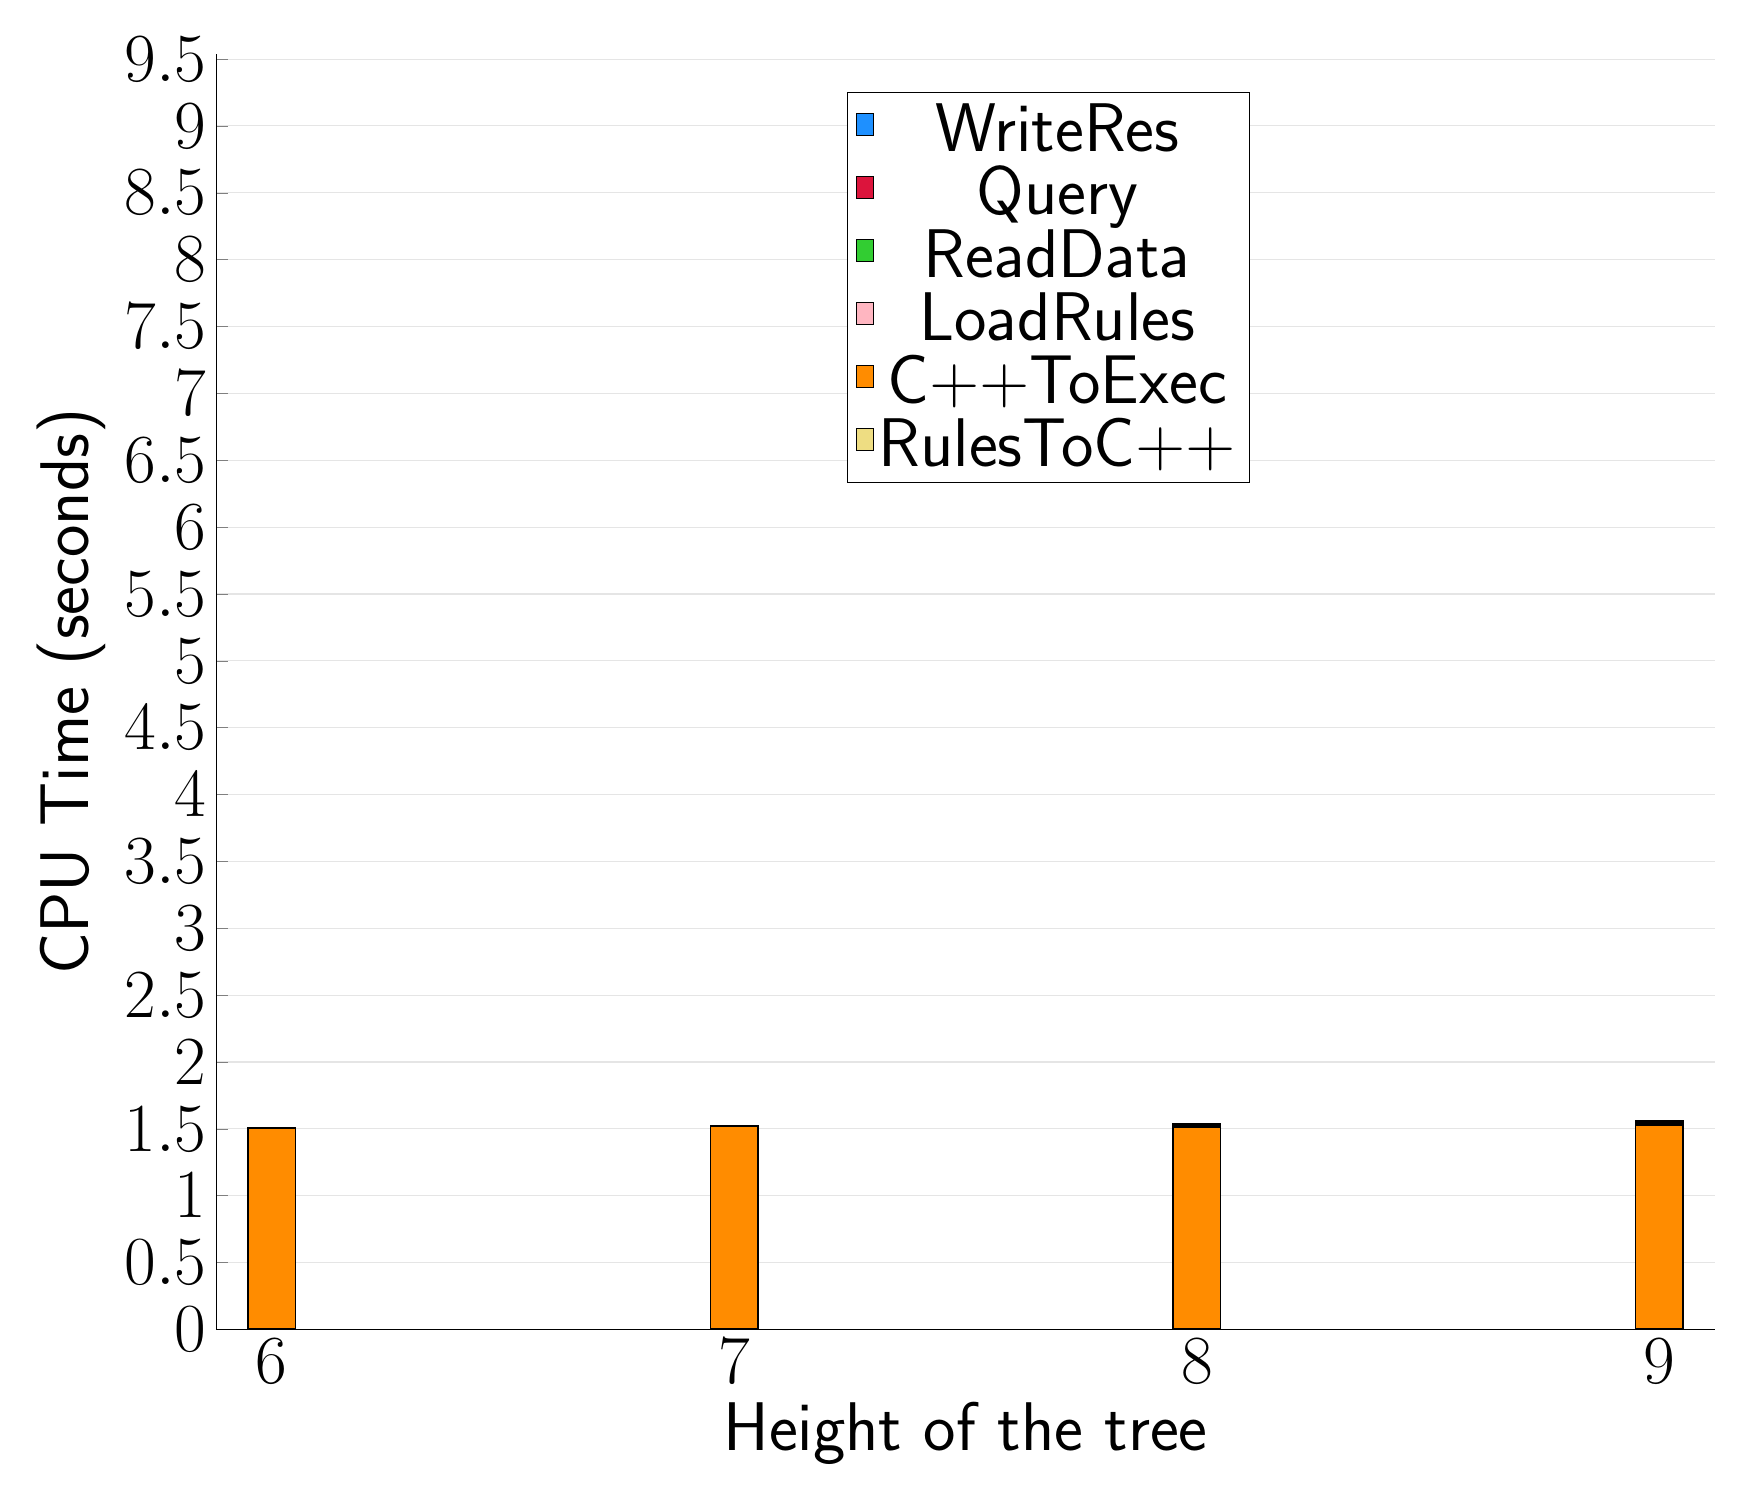
\begin{tikzpicture}
\begin{axis}[
   ybar stacked,
   width=1.7\textwidth,
   bar width=0.6cm,
   ymajorgrids, tick align=inside,
   major grid style={draw=gray!20},
   xtick=data,
   ymin=0, ymax=9.538,
   axis x line*=bottom,
   axis y line*=left,
   enlarge x limits=0.04,
   legend style={
       at={(0.69, 0.97)},
       anchor=north east,
       legend columns=1,
       font=\Huge,
   },
   ylabel={CPU Time (seconds)},
   xlabel={Height of the tree},
   label style={font=\Huge},
   tick label style={font=\Huge},
]
\addlegendimage{fill=DodgerBlue, draw=black, line width=0.2pt}
\addlegendentry{WriteRes}
\addlegendimage{fill=Crimson, draw=black, line width=0.2pt}
\addlegendentry{Query}
\addlegendimage{fill=LimeGreen, draw=black, line width=0.2pt}
\addlegendentry{ReadData}
\addlegendimage{fill=LightPink, draw=black, line width=0.2pt}
\addlegendentry{LoadRules}
\addlegendimage{fill=DarkOrange, draw=black, line width=0.2pt}
\addlegendentry{C++ToExec}
\addlegendimage{fill=LightGoldenrod, draw=black, line width=0.2pt}
\addlegendentry{RulesToC++}
\addplot +[fill=LightGoldenrod, draw=black, line width=0.55pt] coordinates {
(6, 0.0020000000000000005)
(7, 0.006000000000000001)
(8, 0.0020000000000000005)
(8, 0.0020000000000000005)
(8, 0.0020000000000000005)
(9, 0.004000000000000001)
(9, 0.0)
(9, 0.0)
(9, 0.0)
(9, 0.0)
};
\addplot +[fill=DarkOrange, draw=black, line width=0.55pt] coordinates {
(6, 1.5059999999999998)
(7, 1.512)
(8, 1.5100000000000002)
(8, 1.5239999999999998)
(8, 1.516)
(9, 1.538)
(9, 1.528)
(9, 1.53)
(9, 1.5320000000000003)
(9, 1.536)
};
\addplot +[fill=LightPink, draw=black, line width=0.55pt] coordinates {
(6, 0.000165)
(7, 0.0001576)
(8, 0.0001406)
(8, 0.0001604)
(8, 0.0001224)
(9, 9.24e-05)
(9, 0.00016060000000000003)
(9, 0.00015999999999999999)
(9, 0.0001602)
(9, 0.00016040000000000002)
};
\addplot +[fill=LimeGreen, draw=black, line width=0.55pt] coordinates {
(6, 0.0006328)
(7, 0.0007744)
(8, 0.0010092)
(8, 0.0011474)
(8, 0.0009288000000000001)
(9, 0.0015024)
(9, 0.0023006)
(9, 0.0023792)
(9, 0.0023744)
(9, 0.0024942)
};
\addplot +[fill=Crimson, draw=black, line width=0.55pt] coordinates {
(6, 0.0011546)
(7, 0.0030758)
(8, 0.0062418000000000005)
(8, 0.0070882)
(8, 0.0061046)
(9, 0.0152814)
(9, 0.017874)
(9, 0.017854599999999998)
(9, 0.0175332)
(9, 0.018003799999999997)
};
\addplot +[fill=DodgerBlue, draw=black, line width=0.55pt] coordinates {
(6, 0.00011040000000000001)
(7, 0.0001224)
(8, 7.34e-05)
(8, 8.400000000000001e-05)
(8, 4.2000000000000004e-05)
(9, 5.08e-05)
(9, 0.0001338)
(9, 0.00011219999999999999)
(9, 0.0001428)
(9, 0.00014120000000000002)
};
\end{axis}
\end{tikzpicture}

\end{document}
